\section*{Trace 7: Symbolic Reflection in Diabetes Dataset}
\label{section:trace7_symbolic_reflection_diabetes}

\begin{figure}[htbp]
\centering
\caption[\textit{SRV trace (summary)}]{%
\parbox{0.9\linewidth}{\centering
\textit{This SRV trace extends the behavior established in Trace~5, further illustrating the symbolic dynamics of Definition~ through derivative visualization.}
}}
\label{figure:trace7_summary_diabetes}
\end{figure}

\subsection*{1 Objective}
\label{subsection:trace7_objective}

Trace symbolic flow coherence and sparsity transitions within the scikit-learn Diabetes dataset. This instance reflects an observer-bound echo of Trace 5’s synthetic patterning.

\subsection*{2 Validation Setup}
\label{subsection:trace7_validation_setup}

Lp regression was applied across $p \in \{1.0, 1.2, \ldots, 2.0\}$ using the Diabetes dataset. Metrics:
\begin{itemize}
    \item \textbf{Residual Error:} Mean absolute error trend
    \item \textbf{Sparsity:} Feature selection strength across $p$
\end{itemize}

\subsection*{3 Symbolic Responses and Figures}
\label{subsection:trace7_symbolic_responses_figures}

\begin{figure}[htbp]
\centering
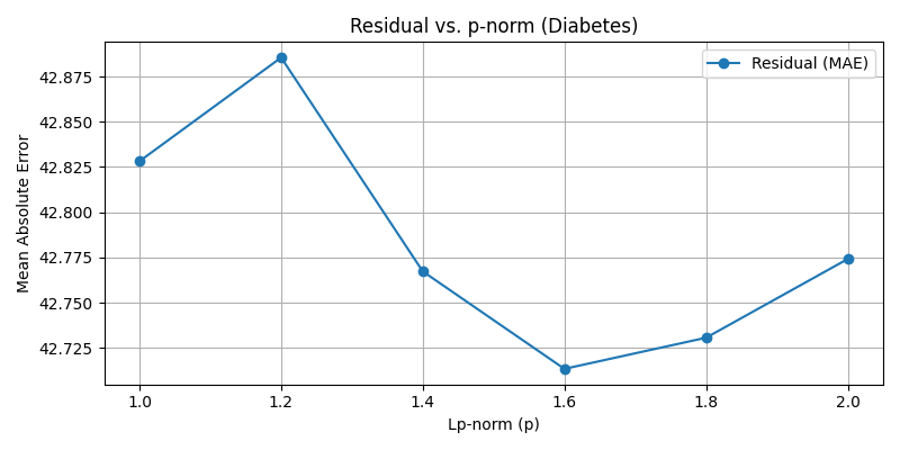
\includegraphics[width=0.85\textwidth]{srv_traces/7_residual_vs_p.png}
\caption{Residual MAE vs. Lp-norm on Diabetes dataset}
\label{figure:trace7_residual_mae_diabetes}
\end{figure}

\begin{figure}[htbp]
\centering
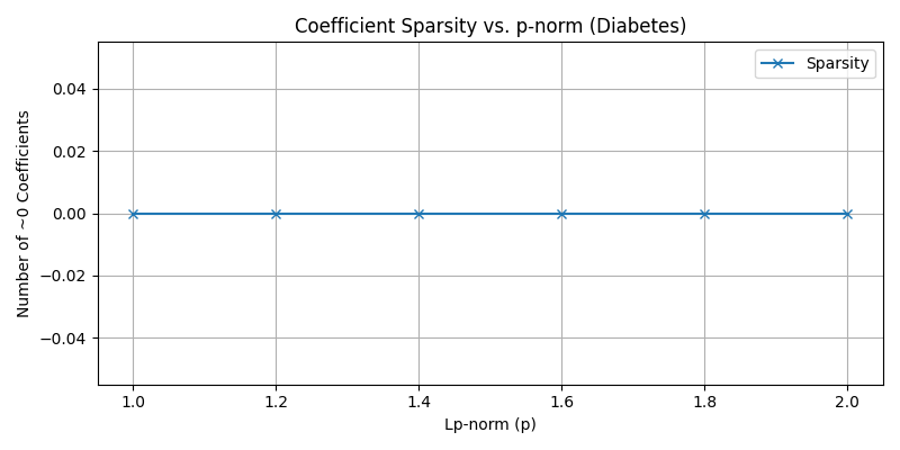
\includegraphics[width=0.85\textwidth]{srv_traces/7_sparsity_vs_p.png}
\caption{Sparsity vs. Lp-norm on Diabetes dataset}
\label{figure:trace7_sparsity_diabetes}
\end{figure}

\subsection*{4 Conclusion}
\label{subsection:trace7_conclusion}

Drift–reflection principles manifest coherently under bounded symbolic constraints. Observed sparsity and residual trajectories align with symbolic emergence, suggesting that symbolic structure propagates consistently across manifold membranes.

\subsection*{5 Theory Linkage}
\label{subsection:trace7_theory_linkage}

\begin{itemize}
    \item \textbf{Theorem 2.2:} Symbolic Entropy and Drift
    \item \textbf{Corollary 7.2:} Recursive Convergence Principle
    \item \textbf{Book IX Themes:} Symbolic agency and constraint
\end{itemize}
